\begin{comment}
Automatic translation from CWP and BPMN to LTL properties and Promela code, respectively, is not trivial. First, the edges of the CWP must follow a consistent expression language in order to be interpreted automatically. Next, the object state must be clearly defined. Also, several implied BPMN semantics lead to ambiguous workflow structures, requiring additional automated reasoning. Next, the complete conditions of decision gateways in the workflow must be expressed somewhere. Finally, the environment for running the workflow must be defined, including variables and behavior models for BPMN activities.
\end{comment}

\figref{fig:newSolutionRoadmap} shows a diagram of our improved solution for verifying BPMNs against CWPs. It is an improvement upon the solution represented by \figref{fig:existingSolution}. The elements that are new additions to the solution are colored teal. One of the primary advantages of the new solution is that almost the entire translation and verification processes are automated.

Automatic translation from CWP and BPMN to LTL properties and Promela code, respectively, is not trivial. First, a standard of CWP construction must be established such that the diagram can be consistently interpreted and ingested by the automation tool. There is also the problem of BPMN interpretation and ingestion. Some information in BPMN diagrams requires standardization in order to convert directly to valid Promela code. Also, several implied BPMN semantics lead to ambiguous workflow structures, requiring additional automated reasoning. Next, the object state must be clearly defined. Finally, the specifics of how each activity in the BPMN affects the object state must be defined. These requirements lead to two additional files being required for verification in addition to the XML files for borh the CWP and BPMN diagrams. The details of these two files will be given in \secref{sec:envConstruction}.

\begin{figure*}[t]
  \begin{center}
    \begin{tabular}{c}
        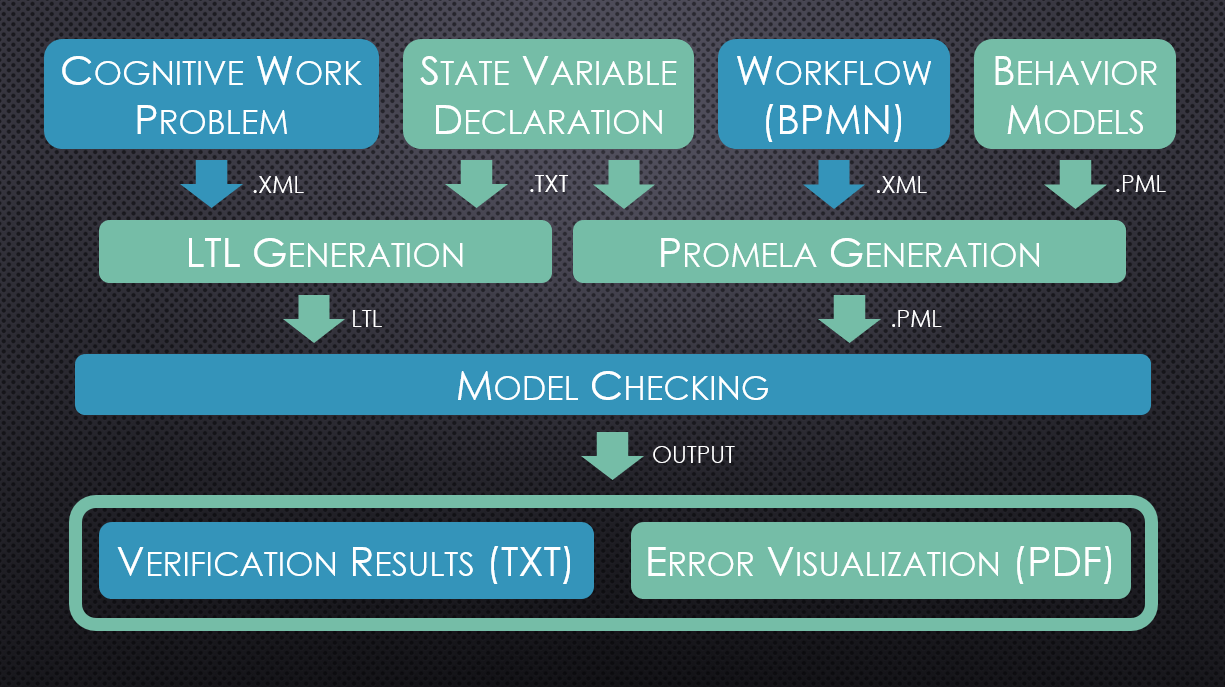
\includegraphics[width=\textwidth]{../figs/Other/NewSolutionRoadmap.png}
    \end{tabular}
  \end{center}
\caption{Diagram of the automated BPMN verification solution. New elements are colored teal.}
\label{fig:newSolutionRoadmap}
\end{figure*}
